\documentclass[12pt]{article}
\usepackage{pgfplots}
\usepgfplotslibrary{groupplots}
\usepackage{multirow}
\pgfplotsset{compat=1.18}
\usepackage{graphicx}
\usepackage{amsmath} 
\usepackage{ragged2e}
\usepackage{amssymb}
\usepackage{float}
\usepackage{mathabx}
\usepackage{mathtools}
\usepackage{tikz}
\usepackage{tikz-3dplot}
\usepackage{caption}
\usepackage[makeroom]{cancel}
\usepackage{biblatex} 
\usepackage{amsfonts}
\usepackage{url}
\usepackage{gensymb}
\usepackage{mathrsfs}
\usepackage{titling}
\usepackage{circuitikz}
\addbibresource{citations.bib}
\newcommand{\subtitle}[1]{
  \posttitle{
    \par\end{center}
    \begin{center}\large#1\end{center}
    \vskip0.5em
  }
}

\newtheorem{theorem}{Theorem}

\title{Electromagnetic Force Symmetry}
\author{Giovani Mendes Crepaldi}
\date{August 2026}

\begin{document}

\maketitle

\section{Introduction}
\subsection{Motivation}
The main motivation for proposing the conjecture was the following problem:
Given a constant linear charge density $\lambda$ on an infinite length charged bar, describe the resulting electrical field on the point P.

\begin{center}
    \begin{tikzpicture}[>=stealth, scale=1.2]
    \draw[->, thick] (-1, 0) -- (4.5, 0) node[right] {$x$};
    \draw[->, thick] (0, -3.5) -- (0, 3.5) node[above] {$y$};
    
    \node[below left] at (0,0) {$O$};

    \draw[line width=1.5pt, blue!70!black] (0, -3.2) -- (0, 3.2);
    
    \node[blue!70!black, above] at (0, 3.2) {$\vdots$};
    \node[blue!70!black, below] at (0, -3.2) {$\vdots$};

    \coordinate (P) at (3, 0);
    \filldraw[red!80!black] (P) circle (2pt) node[above right] {$P$};

    \draw[<->, dashed, color=gray!80!black] (0, -0.4) -- (3, -0.4) node[midway, below] {$P$ (distance)};

    \node[blue!70!black, align=left, anchor=east] at (-0.3, 1.5) {$\lambda = \text{constant}$\\(linear density\\electrical charge)};

    \draw[ultra thick, red!60!black] (0, 1.2) -- (0, 1.5) node[midway, left=2pt] {\footnotesize $dy$};
    \draw[dotted, gray] (0, 1.35) -- (P);
    \draw[->, thick, red!70!black] (P) -- (3.8, -0.36) node[right] {$d\mathbf{E}$};
    \node[above right, font=\footnotesize] at (1.5, 0.67) {$r = \sqrt{x^2 + y^2}$};
    
\end{tikzpicture}
\end{center}

The idea behind the solution is that, for every $dy$ on the bar's length there is a $dE$ contribution to the resulting electrical field, but because the bar's length is infinite, for every charge element $dy$ such that $dq=\lambda dy$ on the positive y-axis, there exists a charge element $-dy$ on the negative y-axis such that the vertical component of the resulting forces cancel each other out, and the resulting electrical field on the point such that $\mid E\mid<\infty$.
Also, note that, since only the vertical components have been canceled, the horizontal components remain and actually add up:
\[dE_+=dE_x\hat{x}+dE_y\hat{y}\]
\[dE_-=dE_x\hat{x}-dE_y\hat{y}\]
\[\therefore dE_+ +dE_-=2dE_x\hat{x}\]
You can solve the problem for yourself, but solving it yields the natural question:
Under what conditions can symmetry-induced vector-component cancellations be consistently applied to other configurations?

\subsection{Generalization}
The previous problem contains a simple geometric structure that is useful for generalization. The charged source extends to infinity in one spatial direction, while the point at which the electric field is evaluated has zero geometric dimensions. Let $D$ be the dimension of the Euclidean space in which the configuration is embedded. For the example above, $D=2$, since only two spatial coordinates are required to describe the configuration. Let $k$ denote the number of spatial directions in which the source is infinite. Here, $k=1$.

Observe in this example that the symmetry cancels the components parallel to the unbounded direction, leaving only the perpendicular x components.

Also, note that the purpose of the analysis isn't to determine the total force acting on an infinitely extended body. Instead, we are interested in the local electromagnetic interaction on each point of the affected body. 

For an extended charged body, this distinction can be expressed in terms of the local density. For a surface charge density $\lambda$, for example,

\[
d\mathbf F = \lambda \mathbf E\,dA,
\]

so that

\[
\frac{d\mathbf F}{dA}=\lambda\mathbf E.
\]

Although the total force obtained by integrating this quantity over an infinitely extended surface diverges,

\[
\mathbf F = \int_{\mathbb R^2} \lambda\mathbf E\,dA,
\]
the local field $\mathbf E$ and, consequently, the local force density $d\mathbf F/dA$ may remain finite.
\par
We can further observe these relations on some other well-known problems involving similar configurations, given:

\tdplotsetmaincoords{20}{110}
\begin{center}
\begin{tikzpicture}[tdplot_main_coords, scale=0.85, every node/.style={scale=0.85}, >=stealth]

    \draw[->, thick, gray!50] (-2.5,0,0) -- (5.5,0,0) node[anchor=north east]{$x$};
    \draw[->, thick, gray!50] (0,-4,0) -- (0,4.5,0) node[anchor=north west]{$y$};
    \draw[->, thick, gray!50] (0,0,-4.5) -- (0,0,5.5) node[anchor=south]{$z$};

    \fill[blue!20, opacity=0.55] (0, -3.5, -3.5) -- (0, 3.5, -3.5) -- (0, 3.5, 3.5) -- (0, -3.5, 3.5) -- cycle;
    \draw[blue!80!black, line width=1.1pt] (0, -3.5, -3.5) -- (0, 3.5, -3.5) -- (0, 3.5, 3.5) -- (0, -3.5, 3.5) -- cycle;

    \draw[blue!80!black, dashed, thick] (0, 3.5, 0) -- (0, 4.8, 0);
    \draw[blue!80!black, dashed, thick] (0, -3.5, 0) -- (0, -4.8, 0);
    \draw[blue!80!black, dashed, thick] (0, 0, 3.5) -- (0, 0, 4.8);
    \draw[blue!80!black, dashed, thick] (0, 0, -3.5) -- (0, 0, -4.8);

    \node[blue!90!black, font=\small, anchor=south west] at (0, 1, 3.5) {Body};

    \draw[<->, thick, dashed, color=black!70] (0, 0, -0.5) -- (1.5, 0, -0.5) node[midway, below, font=\small] {$d$};
    
    \draw[<->, thick, color=black!80] (1.5, -2.5, -3) -- (4, -2.5, -3) node[midway, below, font=\small] {$L$};
    \draw[dotted, gray!70] (1.5,-2.5,-2.5) -- (1.5,-2.5,-3.2);
    \draw[dotted, gray!70] (4,-2.5,-2.5) -- (4,-2.5,-3.2);

    \fill[orange!30, opacity=0.6] (1.5,-2.5,-2.5) -- (1.5,2.5,-2.5) -- (1.5,2.5,2.5) -- (1.5,-2.5,2.5) -- cycle;
    \draw[red!80!black, line width=1.2pt] (1.5,-2.5,-2.5) -- (1.5,2.5,-2.5) -- (1.5,2.5,2.5) -- (1.5,-2.5,2.5) -- cycle;

    \fill[orange!40, opacity=0.5] (1.5,2.5,-2.5) -- (4,2.5,-2.5) -- (4,2.5,2.5) -- (1.5,2.5,2.5) -- cycle;
    \fill[orange!50, opacity=0.6] (1.5,-2.5,2.5) -- (4,-2.5,2.5) -- (4,2.5,2.5) -- (1.5,2.5,2.5) -- cycle;

    \fill[orange!35, opacity=0.7] (4,-2.5,-2.5) -- (4,2.5,-2.5) -- (4,2.5,2.5) -- (4,-2.5,2.5) -- cycle;
    \draw[red!80!black, line width=1.2pt] (4,-2.5,-2.5) -- (4,2.5,-2.5) -- (4,2.5,2.5) -- (4,-2.5,2.5) -- cycle;

    \draw[red!80!black, line width=1.2pt] (1.5,2.5,2.5) -- (4,2.5,2.5);
    \draw[red!80!black, line width=1.2pt] (1.5,-2.5,2.5) -- (4,-2.5,2.5);
    \draw[red!80!black, line width=1.2pt] (1.5,2.5,-2.5) -- (4,2.5,-2.5);
    \draw[red!80!black, line width=1.2pt] (1.5,-2.5,-2.5) -- (4,-2.5,-2.5);

    \draw[red!80!black, dashed, thick] (1.5,2.5,0) -- (1.5,4.2,0);
    \draw[red!80!black, dashed, thick] (1.5,-2.5,0) -- (1.5,-4.2,0);
    \draw[red!80!black, dashed, thick] (4,2.5,0) -- (4,4.2,0);
    \draw[red!80!black, dashed, thick] (4,-2.5,0) -- (4,-4.2,0);

    \draw[red!80!black, dashed, thick] (1.5,0,2.5) -- (1.5,0,4.2);
    \draw[red!80!black, dashed, thick] (1.5,0,-2.5) -- (1.5,0,-4.2);
    \draw[red!80!black, dashed, thick] (4,0,2.5) -- (4,0,4.2);
    \draw[red!80!black, dashed, thick] (4,0,-2.5) -- (4,0,-4.2);

    \node[red!80!black, font=\small, anchor=south west] at (2.2, 1.5, 2.7) {Source};

\end{tikzpicture}
\end{center}

Here, $D=3$, and the source is infinite in the $y$ and $z$ directions, so $k=2$.
Note that, if we consider the corresponding cross-sectional representation in $D=2$:

\tdplotsetmaincoords{90}{0}
\begin{center}
\begin{tikzpicture}[tdplot_main_coords, scale=0.85, every node/.style={scale=0.85}, >=stealth]

    \draw[->, thick, gray!50] (-2.5,0,0) -- (5.5,0,0) node[anchor=north east]{$x$};
    \draw[->, thick, gray!50] (0,-4,0) -- (0,4.5,0) node[anchor=north west]{$y$};
    \draw[->, thick, gray!50] (0,0,-4.5) -- (0,0,5.5) node[anchor=south]{$z$};

    \fill[blue!20, opacity=0.55] (0, -3.5, -3.5) -- (0, 3.5, -3.5) -- (0, 3.5, 3.5) -- (0, -3.5, 3.5) -- cycle;
    \draw[blue!80!black, line width=1.1pt] (0, -3.5, -3.5) -- (0, 3.5, -3.5) -- (0, 3.5, 3.5) -- (0, -3.5, 3.5) -- cycle;

    \draw[blue!80!black, dashed, thick] (0, 3.5, 0) -- (0, 4.8, 0);
    \draw[blue!80!black, dashed, thick] (0, -3.5, 0) -- (0, -4.8, 0);
    \draw[blue!80!black, dashed, thick] (0, 0, 3.5) -- (0, 0, 4.8);
    \draw[blue!80!black, dashed, thick] (0, 0, -3.5) -- (0, 0, -4.8);

    \node[blue!90!black, font=\small, anchor=south west] at (0, 1, 3.5) {Body};

    \draw[<->, thick, dashed, color=black!70] (0, 0, -0.5) -- (1.5, 0, -0.5) node[midway, below, font=\small] {$d$};
    
    \draw[<->, thick, color=black!80] (1.5, -2.5, -3) -- (4, -2.5, -3) node[midway, below, font=\small] {$L$};
    \draw[dotted, gray!70] (1.5,-2.5,-2.5) -- (1.5,-2.5,-3.2);
    \draw[dotted, gray!70] (4,-2.5,-2.5) -- (4,-2.5,-3.2);

    \fill[orange!30, opacity=0.6] (1.5,-2.5,-2.5) -- (1.5,2.5,-2.5) -- (1.5,2.5,2.5) -- (1.5,-2.5,2.5) -- cycle;
    \draw[red!80!black, line width=1.2pt] (1.5,-2.5,-2.5) -- (1.5,2.5,-2.5) -- (1.5,2.5,2.5) -- (1.5,-2.5,2.5) -- cycle;

    \fill[orange!40, opacity=0.5] (1.5,2.5,-2.5) -- (4,2.5,-2.5) -- (4,2.5,2.5) -- (1.5,2.5,2.5) -- cycle;
    \fill[orange!50, opacity=0.6] (1.5,-2.5,2.5) -- (4,-2.5,2.5) -- (4,2.5,2.5) -- (1.5,2.5,2.5) -- cycle;

    \fill[orange!35, opacity=0.7] (4,-2.5,-2.5) -- (4,2.5,-2.5) -- (4,2.5,2.5) -- (4,-2.5,2.5) -- cycle;
    \draw[red!80!black, line width=1.2pt] (4,-2.5,-2.5) -- (4,2.5,-2.5) -- (4,2.5,2.5) -- (4,-2.5,2.5) -- cycle;

    \draw[red!80!black, line width=1.2pt] (1.5,2.5,2.5) -- (4,2.5,2.5);
    \draw[red!80!black, line width=1.2pt] (1.5,-2.5,2.5) -- (4,-2.5,2.5);
    \draw[red!80!black, line width=1.2pt] (1.5,2.5,-2.5) -- (4,2.5,-2.5);
    \draw[red!80!black, line width=1.2pt] (1.5,-2.5,-2.5) -- (4,-2.5,-2.5);

    \draw[red!80!black, dashed, thick] (1.5,2.5,0) -- (1.5,4.2,0);
    \draw[red!80!black, dashed, thick] (1.5,-2.5,0) -- (1.5,-4.2,0);
    \draw[red!80!black, dashed, thick] (4,2.5,0) -- (4,4.2,0);
    \draw[red!80!black, dashed, thick] (4,-2.5,0) -- (4,-4.2,0);

    \draw[red!80!black, dashed, thick] (1.5,0,2.5) -- (1.5,0,4.2);
    \draw[red!80!black, dashed, thick] (1.5,0,-2.5) -- (1.5,0,-4.2);
    \draw[red!80!black, dashed, thick] (4,0,2.5) -- (4,0,4.2);
    \draw[red!80!black, dashed, thick] (4,0,-2.5) -- (4,0,-4.2);

    \node[red!80!black, font=\small, anchor=south west] at (2.2, 1.5, 2.7) {Source};

\end{tikzpicture}
\end{center}

Other example:

\tdplotsetmaincoords{20}{110}
\begin{center}
\begin{tikzpicture}[tdplot_main_coords, scale=0.85, every node/.style={scale=0.85}, >=stealth]

    \draw[->, thick, gray!50] (-2.5,0,0) -- (5.5,0,0) node[anchor=north east]{$x$};
    \draw[->, thick, gray!50] (0,-4,0) -- (0,4.5,0) node[anchor=north west]{$y$};
    \draw[->, thick, gray!50] (0,0,-4.5) -- (0,0,5.5) node[anchor=south]{$z$};

    \draw[line width=2pt, blue!70!black] (0,0,-3.5) -- (0,0,3.5);
    \draw[blue!70!black, dashed, line width=1.5pt] (0,0,3.5) -- (0,0,4.8);
    \draw[blue!70!black, dashed, line width=1.5pt] (0,0,-3.5) -- (0,0,-4.8);
    
    \node[blue!80!black, above] at (0,0,4.8) {$\vdots$};
    \node[blue!80!black, below] at (0,0,-4.8) {$\vdots$};
    \node[blue!90!black, font=\small, anchor=east] at (-0.3, 0, 3) {Body};

    \draw[<->, thick, dashed, color=black!70] (0, 0, -0.5) -- (1.5, 0, -0.5) node[midway, below, font=\small] {$d$};
    
    \draw[<->, thick, color=black!80] (1.5, -2.5, -3) -- (4, -2.5, -3) node[midway, below, font=\small] {$L$};
    \draw[dotted, gray!70] (1.5,-2.5,-2.5) -- (1.5,-2.5,-3.2);
    \draw[dotted, gray!70] (4,-2.5,-2.5) -- (4,-2.5,-3.2);

    \fill[orange!30, opacity=0.6] (1.5,-2.5,-2.5) -- (1.5,2.5,-2.5) -- (1.5,2.5,2.5) -- (1.5,-2.5,2.5) -- cycle;
    \draw[red!80!black, line width=1.2pt] (1.5,-2.5,-2.5) -- (1.5,2.5,-2.5) -- (1.5,2.5,2.5) -- (1.5,-2.5,2.5) -- cycle;

    \fill[orange!40, opacity=0.5] (1.5,2.5,-2.5) -- (4,2.5,-2.5) -- (4,2.5,2.5) -- (1.5,2.5,2.5) -- cycle;
    \fill[orange!50, opacity=0.6] (1.5,-2.5,2.5) -- (4,-2.5,2.5) -- (4,2.5,2.5) -- (1.5,2.5,2.5) -- cycle;

    \fill[orange!35, opacity=0.7] (4,-2.5,-2.5) -- (4,2.5,-2.5) -- (4,2.5,2.5) -- (4,-2.5,2.5) -- cycle;
    \draw[red!80!black, line width=1.2pt] (4,-2.5,-2.5) -- (4,2.5,-2.5) -- (4,2.5,2.5) -- (4,-2.5,2.5) -- cycle;

    \draw[red!80!black, line width=1.2pt] (1.5,2.5,2.5) -- (4,2.5,2.5);
    \draw[red!80!black, line width=1.2pt] (1.5,-2.5,2.5) -- (4,-2.5,2.5);
    \draw[red!80!black, line width=1.2pt] (1.5,2.5,-2.5) -- (4,2.5,-2.5);
    \draw[red!80!black, line width=1.2pt] (1.5,-2.5,-2.5) -- (4,-2.5,-2.5);

    \draw[red!80!black, dashed, thick] (1.5,2.5,0) -- (1.5,4.2,0);
    \draw[red!80!black, dashed, thick] (1.5,-2.5,0) -- (1.5,-4.2,0);
    \draw[red!80!black, dashed, thick] (4,2.5,0) -- (4,4.2,0);
    \draw[red!80!black, dashed, thick] (4,-2.5,0) -- (4,-4.2,0);

    \draw[red!80!black, dashed, thick] (1.5,0,2.5) -- (1.5,0,4.2);
    \draw[red!80!black, dashed, thick] (1.5,0,-2.5) -- (1.5,0,-4.2);
    \draw[red!80!black, dashed, thick] (4,0,2.5) -- (4,0,4.2);
    \draw[red!80!black, dashed, thick] (4,0,-2.5) -- (4,0,-4.2);

    \node[red!80!black, font=\small, anchor=south west] at (2.2, 1.5, 2.7) {Source};

\end{tikzpicture}
\end{center}
Here, $D=3$ and the source is still infinite in two directions ($y$ and $z$), so $k=2$.
If we consider the corresponding cross-sectional representation in $D=2$:

\tdplotsetmaincoords{90}{0}
\begin{center}
\begin{tikzpicture}[tdplot_main_coords, scale=0.85, every node/.style={scale=0.85}, >=stealth]

    \draw[->, thick, gray!50] (-2.5,0,0) -- (5.5,0,0) node[anchor=north east]{$x$};
    \draw[->, thick, gray!50] (0,-4,0) -- (0,4.5,0) node[anchor=north west]{$y$};
    \draw[->, thick, gray!50] (0,0,-4.5) -- (0,0,5.5) node[anchor=south]{$z$};

    \draw[line width=2pt, blue!70!black] (0,0,-3.5) -- (0,0,3.5);
    \draw[blue!70!black, dashed, line width=1.5pt] (0,0,3.5) -- (0,0,4.8);
    \draw[blue!70!black, dashed, line width=1.5pt] (0,0,-3.5) -- (0,0,-4.8);
    
    \node[blue!80!black, above] at (0,0,4.8) {$\vdots$};
    \node[blue!80!black, below] at (0,0,-4.8) {$\vdots$};
    \node[blue!90!black, font=\small, anchor=east] at (-0.3, 0, 3) {Body};

    \draw[<->, thick, dashed, color=black!70] (0, 0, -0.5) -- (1.5, 0, -0.5) node[midway, below, font=\small] {$d$};
    
    \draw[<->, thick, color=black!80] (1.5, -2.5, -3) -- (4, -2.5, -3) node[midway, below, font=\small] {$L$};
    \draw[dotted, gray!70] (1.5,-2.5,-2.5) -- (1.5,-2.5,-3.2);
    \draw[dotted, gray!70] (4,-2.5,-2.5) -- (4,-2.5,-3.2);

    \fill[orange!30, opacity=0.6] (1.5,-2.5,-2.5) -- (1.5,2.5,-2.5) -- (1.5,2.5,2.5) -- (1.5,-2.5,2.5) -- cycle;
    \draw[red!80!black, line width=1.2pt] (1.5,-2.5,-2.5) -- (1.5,2.5,-2.5) -- (1.5,2.5,2.5) -- (1.5,-2.5,2.5) -- cycle;

    \fill[orange!40, opacity=0.5] (1.5,2.5,-2.5) -- (4,2.5,-2.5) -- (4,2.5,2.5) -- (1.5,2.5,2.5) -- cycle;
    \fill[orange!50, opacity=0.6] (1.5,-2.5,2.5) -- (4,-2.5,2.5) -- (4,2.5,2.5) -- (1.5,2.5,2.5) -- cycle;

    \fill[orange!35, opacity=0.7] (4,-2.5,-2.5) -- (4,2.5,-2.5) -- (4,2.5,2.5) -- (4,-2.5,2.5) -- cycle;
    \draw[red!80!black, line width=1.2pt] (4,-2.5,-2.5) -- (4,2.5,-2.5) -- (4,2.5,2.5) -- (4,-2.5,2.5) -- cycle;

    \draw[red!80!black, line width=1.2pt] (1.5,2.5,2.5) -- (4,2.5,2.5);
    \draw[red!80!black, line width=1.2pt] (1.5,-2.5,2.5) -- (4,-2.5,2.5);
    \draw[red!80!black, line width=1.2pt] (1.5,2.5,-2.5) -- (4,2.5,-2.5);
    \draw[red!80!black, line width=1.2pt] (1.5,-2.5,-2.5) -- (4,-2.5,-2.5);

    \draw[red!80!black, dashed, thick] (1.5,2.5,0) -- (1.5,4.2,0);
    \draw[red!80!black, dashed, thick] (1.5,-2.5,0) -- (1.5,-4.2,0);
    \draw[red!80!black, dashed, thick] (4,2.5,0) -- (4,4.2,0);
    \draw[red!80!black, dashed, thick] (4,-2.5,0) -- (4,-4.2,0);

    \draw[red!80!black, dashed, thick] (1.5,0,2.5) -- (1.5,0,4.2);
    \draw[red!80!black, dashed, thick] (1.5,0,-2.5) -- (1.5,0,-4.2);
    \draw[red!80!black, dashed, thick] (4,0,2.5) -- (4,0,4.2);
    \draw[red!80!black, dashed, thick] (4,0,-2.5) -- (4,0,-4.2);

    \node[red!80!black, font=\small, anchor=south west] at (2.2, 1.5, 2.7) {Source};

\end{tikzpicture}
\end{center}
We will show that, for this configuration, we can quickly verify that the local electric field remains finite. This example was chosen over the previous example because it represents a more non trivial configuration, showing that the dimension reduction could play a big part in recognizing convergence in local electrical fields.
Consider the source described by:
\[0\leq x \leq L:x\qquad x,L\in \mathbb{R} \quad \mid L\mid <\infty\]
\[y,z\in \mathbb{R}\]

And with uniform volume charge density $\rho$. The affected body is taken to be an infinitely extended line, aligned with one of the directions of infinite extent of the source and located outside the source. Here, $D=3$ and $k=2$.
The local electric field can be described by decomposing the source in planes perpendicular to the $x$-axis. Each plane is infinite in the $y$ and $z$ directions and has a differential surface charge density
\[
d\sigma=\rho\,dx.
\]
Due to the symmetry of each plane, the components parallel to the plane cancel pairwise, leaving only the component normal to it:
\[
d\mathbf{E}=dE_x\,\hat{\mathbf{x}}.
\]

The magnitude of the remaining component is proportional to the surface charge density of the infinitesimal plane,
\[
dE_x\propto d\sigma.
\]

Therefore,
\[
dE_x\propto \rho\,dx.
\]
Integrating over the finite extent of the source in the $x$-direction then gives
\[
E_x\propto \int_0^L \rho\,dx = \rho L.
\]

Since $L<\infty$ and $\rho$ is assumed finite, it follows that
\[
\boxed{|E_{\mathrm{local}}|<\infty}.
\]

This example DOES NOT mean that symmetry-induced dimensional reduction is always possible, note the simple counter example that shows that there are cases in which the available dimensions are not sufficient to eliminate all contributions to the local electric field.
\[
0\leq x<\infty,
\qquad
y,z\in\mathbb{R},
\]
\footnote{The example simply consists of making the source's dimension $L\rightarrow\infty$}
Consider a source described by
Here, the source is infinite in all three directions, so $D=3$ and $k=3$. In this case, the source is unbounded in all directions. And each plane has a differential surface charge density $d\sigma = \rho\,dx$. Since the electric field of an infinite plane does not depend on its distance to it(an intuition for this it that, moving the point further from the plane is basically the same as zooming out perspectively, and thus the distances does not matter):
\[
dE \propto d\sigma = \rho\,dx
\]
Integrating this over the infinite extent of the source in the $x$-direction gives:
\[
E \propto \int_0^\infty \rho\,dx
\]
Since $\rho$ is assumed finite and $\neq 0$, this integral diverges to infinity. The local field is infinite.

Note that in the finite box example ($D=3, k=2$), the field was finite. Here, in the half-space ($D=3, k=3$), it diverges. That suggests that the falloff of the electric field is tied to the embedding dimension $D$, and the growth of the source's volume is tied to the number of unbounded dimensions, $k$. The relationship governing convergence could be some sort of interplay between $D$ and $k$. 
\[\]
We can formalize this intuition as a practical criterion:\\
\begin{conjecture}[Symmetry-Induced Convergence Bound]
\label{thm:convergence}
\\
Let a charged source be unbounded in $k$ orthogonal spatial directions within an embedding space of dimension $D$. Such that the body of analysis does not lie in the source itself. By symmetry, the parallel components of the local electric field vanish. The remaining perpendicular field is finite if and only if:
\[
\boxed{k \leq D - 1}
\]
\end{conjecture}

\subsection{Towards a "Proof"}


\[\]

As a visualization of what's happening, imagine a source that is infinite in $k$ directions. If $k = D$, the source either is unbalanced relative to the body, making the forces not cancel each other(case 1) or occupies the entire space of analysis, which means that the body is in the source itself, and therefore is not eligible for the analysis(case 2).
We can actually visualize this in lower dimensions(here, D=2,k=2)

Case 1:
\begin{center}
    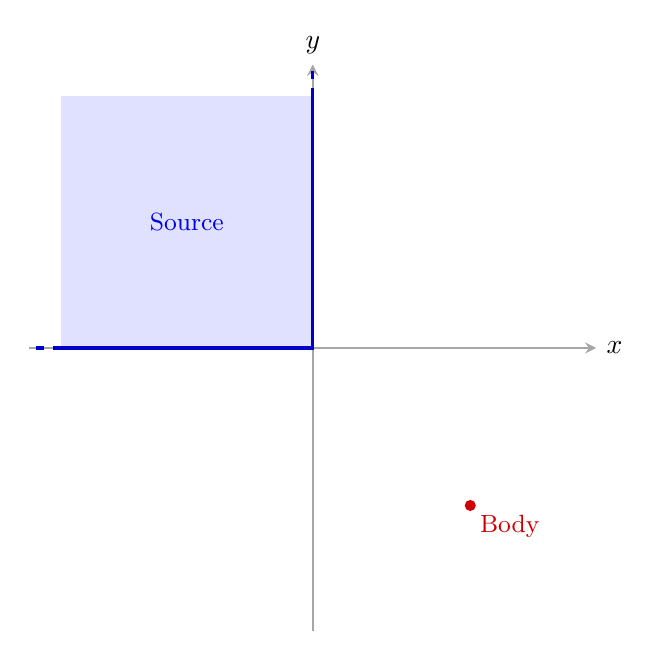
\begin{tikzpicture}[scale=0.8, >=stealth]

    \fill[blue!20, opacity=0.6] (-4,0) -- (0,0) -- (0,4) -- (-4,4) -- cycle;

    \draw[->, thick, gray!70] (-4.5,0) -- (4.5,0) node[right, black]{$x$};
    \draw[->, thick, gray!70] (0,-4.5) -- (0,4.5) node[above, black]{$y$};

    \draw[blue!80!black, line width=1.2pt] (-4,0) -- (0,0) -- (0,4);
    \draw[blue!80!black, dashed, line width=1.2pt] (-4,0) -- (-4.5,0);
    \draw[blue!80!black, dashed, line width=1.2pt] (0,4) -- (0,4.5);

    \node[blue!90!black, font=\small] at (-2,2) {Source};

    \fill[red!80!black] (2.5,-2.5) circle (2.5pt);
    \node[red!80!black, anchor=north west, font=\small] at (2.5,-2.5) {Body};

\end{tikzpicture}
\end{center}
Case 2:
\begin{center}
    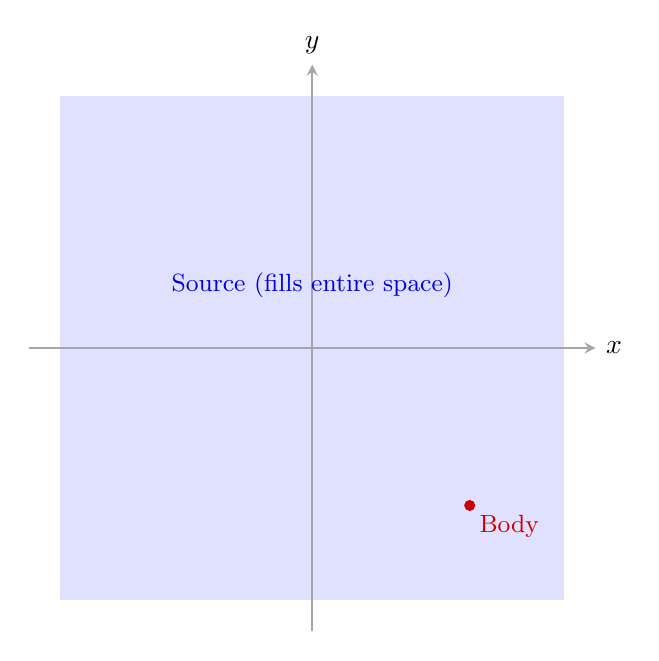
\begin{tikzpicture}[scale=0.8, >=stealth]

    \fill[blue!20, opacity=0.6] (-4,-4) -- (4,-4) -- (4,4) -- (-4,4) -- cycle;

    \draw[->, thick, gray!70] (-4.5,0) -- (4.5,0) node[right, black]{$x$};
    \draw[->, thick, gray!70] (0,-4.5) -- (0,4.5) node[above, black]{$y$};

    \node[blue!90!black, font=\small] at (0,1) {Source (fills entire space)};

    \fill[red!80!black] (2.5,-2.5) circle (2.5pt);
    \node[red!80!black, anchor=north west, font=\small] at (2.5,-2.5) {Body};

\end{tikzpicture}
\end{center}


Notice that, for case 2, if we add a degree of freedom by simply making $D>k$, we can reimagine the space in $D=3$. From a bounded perspective (viewing the 3D space edge-on), the geometry looks identical to the 2D case, it is impossible to tell if the body is trapped inside the source or if it has another degree of freedom into a new dimension that is hidden from our view, and since we can only act based on what we see, we always assume they intersect in a 2D view. However, by making $D=3$:
\tdplotsetmaincoords{45}{110}
\begin{center}
    \begin{tikzpicture}[tdplot_main_coords, scale=0.8, every node/.style={scale=0.85}, >=stealth]

    \draw[->, thick, gray!50] (-3.5,0,0) -- (4.5,0,0) node[anchor=north east]{$x$};
    \draw[->, thick, gray!50] (0,-4,0) -- (0,4.5,0) node[anchor=north west]{$y$};
    \draw[->, thick, gray!50] (0,0,-4.5) -- (0,0,5.5) node[anchor=south]{$z$};

    \fill[blue!20, opacity=0.55] (0, -3.5, -3.5) -- (0, 3.5, -3.5) -- (0, 3.5, 3.5) -- (0, -3.5, 3.5) -- cycle;

    \draw[blue!80!black, line width=1.1pt, dashed] (0, -3.5, -3.5) -- (0, 3.5, -3.5) -- (0, 3.5, 3.5) -- (0, -3.5, 3.5) -- cycle;

    \draw[blue!80!black, dashed, thick] (0, 3.5, 0) -- (0, 4.3, 0);
    \draw[blue!80!black, dashed, thick] (0, -3.5, 0) -- (0, -4.3, 0);
    \draw[blue!80!black, dashed, thick] (0, 0, 3.5) -- (0, 0, 4.3);
    \draw[blue!80!black, dashed, thick] (0, 0, -3.5) -- (0, 0, -4.3);

    \draw[blue!80!black, dashed, thick] (0, 3.5, 3.5) -- (0, 4.2, 4.2);
    \draw[blue!80!black, dashed, thick] (0, -3.5, 3.5) -- (0, -4.2, 4.2);
    \draw[blue!80!black, dashed, thick] (0, 3.5, -3.5) -- (0, 4.2, -4.2);
    \draw[blue!80!black, dashed, thick] (0, -3.5, -3.5) -- (0, -4.2, -4.2);


    \fill[blue!90!black] (0,0,0) circle (2.5pt);

    \draw[<->, thick, dashed, color=black!70] (0, 0, -0.5) -- (2.5, 0, -0.5) node[midway, below, font=\small] {$d$};

    \node[blue!90!black, font=\small, anchor=south west] at (0, 1, 3.5) {Source};
    \fill[red!80!black] (2.5,0,0) circle (2.5pt);
    \node[red!80!black, font=\small, anchor=west] at (2.7, 0, 0) {Body};

\end{tikzpicture}
\end{center}
We gain a new perpendicular degree of freedom. This new dimension creates a distance between the source and the evaluation point, making it eligible for analysis.

Mathematically, we can formalize this intuition. Consider the general form of the local electric field in $D$-dimensional Euclidean space:
\[
\mathbf{E}(\mathbf{r}) = C_D \int_S \rho(\mathbf{r}') \frac{\mathbf{r} - \mathbf{r}'}{|\mathbf{r} - \mathbf{r}'|^D} \, d^D r'
\]
where $C_D$ is the $D$-dimensional Coulomb constant. 

\[\]
Because the source is infinite in $k$ directions, we can split our coordinate system in two: a parallel subspace $V_{\parallel}$ (the $k$ infinite directions) and a perpendicular subspace $V_{\perp}$ (the remaining $D-k$ finite directions). 

By symmetry, the field components parallel to $V_{\parallel}$ cancel out entirely, just like the $y$-axis components canceled in the infinite bar problem. We are left only with a perpendicular component, $\mathbf{E}_{\perp}$. 
Since the parallel counterparts cancel each other, the convergence of the integral depends on an equilibrium. As we move further out, the volume of further charges increases, but the individual field contributions decrease. The balance between this increase and decrease relies on some relationship between $k$ and $D$. Intuitively, for the field to be finite, there must be a bound on $D-k$ that ensures the field weakens fast enough to "beat" the growing volume of charge.
\[\]

Let $R$ be the distance measured along the unbounded subspace $V_{\parallel}$. We split our integral into two parts: the contributions from the "close"/"near" charges (up to some large but finite distance) and the contributions from the "far" charges (the tail of the integral, stretching to infinity). 

The "close" charges always sum to a finite value because there is a finite amount of "contributing" space and the distance is always greater than zero(from the initial condition on the conjecture). Then, the only thing that causes the local field to blow up to infinity is the "tail". To determine if the tail decreases fast enough to be finite, we analyze its behavior when $R$ Tends to infinity.
We break it down to two variables:
As we move further out into the $k$ unbounded directions, the volume of the distant charge elements increases, then, the $k$-dimensional volume element grows proportionally to $R^{k-1}$.
The individual contribution of these distant charges in $D$ dimensions must spread over a $D$-dimensional "sphere", so its magnitude weakens proportionally to $\frac{1}{R^{D-1}}$.
Therefore:
\[
|\mathbf{E}_{\perp}| \propto \int_{R_{\text{min}}}^{\infty} \left( \frac{1}{R^{D-1}} \right) R^{k-1} \, dR = \int_{R_{\text{min}}}^{\infty} R^{k - D} \, dR
\]
where $R_{\text{min}} > 0$ is the minimum distance to the source in the parallel subspace(basically, the bound of the near charges).

An integral of the form $\int^{\infty} R^p \, dR$ converges if the power $p$ is strictly less than $-1$. If $p \geq -1$, the integral diverges. 

Applying this rule to our asymptotic integral, the field is finite if and only if:
\[
k - D < -1
\]
Solving this simple inequality gives:
\[
k < D
\]
Since $k$ and $D$ must be integers, $k < D$ is exactly equivalent to:
\[
\boxed{k \leq D - 1}
\]

\end{document}
